\documentclass{beamer}

\usepackage[utf8]{inputenc}

\title[SymEngine \hspace{14em}\insertframenumber/
\inserttotalframenumber]{SymEngine, a fast symbolic manipulation library}

\usepackage{graphicx}
\graphicspath{ {images/} }


\author[O. Čertík, I. Fernando, ...]{Ondřej Čertík, Isuru Fernando, Thilina Rathnayake, Abhinav Agarwal, Sumith Kulal, Abinash Meher, Rajith Vidanaarachchi}

\begin{document}


\begin{frame}
\maketitle
\end{frame}


\begin{frame}{Outline}
\begin{block}{SymEngine}
\begin{itemize}
\item Introduction
\item Features
\item Demo (Python, Ruby, Julia)
\item Why C++, how to write safe code
\item Internals of SymEngine
\item Roadmap for using SymEngine in SymPy
\item Benchmarks
\end{itemize}
\end{block}
\end{frame}


\begin{frame}
\frametitle{Introduction}
\framesubtitle{About SymEngine}
\begin{itemize}
\item Symbolic manipulation library written in C++
\item Started in 2012
\item 35 contributors
\item Part of SymPy organization
\item MIT licensed
\end{itemize}
\end{frame}


\begin{frame}
\frametitle{Introduction}
\framesubtitle{Goals}
\begin{itemize}
\item Be the fastest symbolic manipulation library (opensource or commercial)
\item Serve as the core for SymPy and Sage
\item Serve as the default symbolic manipulation library in other languages
    thanks to thin wrappers (Python, Ruby, Julia, ...)
\end{itemize}
\end{frame}


\begin{frame}
\frametitle{What language to use}
\begin{block}{Problem}
SymPy speed is sometimes insufficient
\begin{itemize}
\item Handling of very large expressions
\item Large calculations using small/medium size expressions
\end{itemize}
\end{block}

\begin{block}{Let's fix that}
\begin{itemize}
\item We tried: pure Python/PyPy, Cython, C
\item Investigated Julia, Rust, Scala, Javascript, ...
\item Chose C++
\end{itemize}
\end{block}
\end{frame}




\begin{frame}
\frametitle{Features}
\begin{itemize}
    \item Core
    \item Elementary Functions
    \item Matrices
    \item Polynomials
    \item Series expansion
\end{itemize}
\end{frame}


\begin{frame}[fragile]
\frametitle{Features}
\framesubtitle{Symbolic differentiation in SymEngine}
\begin{verbatim}
>>> x = Symbol("x")
>>> y = Symbol("y")
>>> r = x*y+x
>>> gamma(r).diff(x)
(1 + y)*gamma(x + x*y)*polygamma(0, x + x*y)
\end{verbatim}
\end{frame}


\begin{frame}
\frametitle{Features}
\end{frame}

\begin{frame}
\frametitle{Why Pure C++}
\begin{itemize}
\item \textbf{Fast} in Release mode, but safe in Debug mode
\item Compiler helps (not as good as Scala or Haskell, but much better than
    Python)
\item Just one language to learn, thus easy to maintain (as opposed to several
    intertwined layers such as C + Cython + Python)
\item Thin wrappers (that core developers do not need to maintain), all functionality in C++
\item Easier to create bindings to other languages like Python, Julia, Ruby and Haskell.
\end{itemize}
\end{frame}

\begin{frame}
\frametitle{Why Pure C++: Fast in Release Mode}
\begin{itemize}
    \item Allows direct memory handling (allocation, deallocation, access)
    \item Allows to tweak how and when things are done
    \item It is possible to go to bare metal
    \item Allows reasonably high level abstractions (simple, maintainable
        code)
\end{itemize}
\end{frame}

\begin{frame}
\frametitle{Why Pure C++: Safe in Debug Mode}
\begin{itemize}
    \item Reference counted pointers \texttt{Teuchos::RCP} (from Trilinos)
    \item Checks for dangling and null pointers (exception is raised)
    \item No raw pointers/references (use \texttt{Ptr} and \texttt{RCP})
    \item Use a safe subset of C++
    \item Few other rules, e.g. how to use \texttt{Ptr} and \texttt{RCP}
          properly
    \item Possible to visually verify in a PR (pull request) review
    \item Hopefully eventually there are plugins to Clang to check
        automatically (since the rules are simple and static)
    \item As fast as raw pointers in Release mode (but it could segfault)
\end{itemize}
    Conclusion: the code cannot segfault or have undefined behavior in Debug
    mode --- always get an exception at runtime, or a compile error.
\end{frame}


\begin{frame}
\frametitle{Internals of SymEngine}
\framesubtitle{Libraries used}
\begin{itemize}
\item Depends on GNU Multiple Precision library (GMP)
\item Optional dependencies include MPFR, MPC, Flint and Piranha
\end{itemize}
\end{frame}


\begin{frame}
\frametitle{Internals of SymEngine}
\framesubtitle{How Add, Mul and Pow works}
\end{frame}


\begin{frame}
\frametitle{Internals of SymEngine}
\framesubtitle{Extensibility using visitor pattern}
\end{frame}


\begin{frame}[fragile]
\frametitle{SymPy, SymEngine and the interface}
\framesubtitle{Using SymPy in SymEngine}
\begin{itemize}
\item
SymEngine will convert any SymPy object to a corresponding SymEngine object before doing any operation

\begin{verbatim}
>>> from symengine import symbols, Add
>>> import sympy
>>> x = symbols("x")
>>> y = sympy.symbols("y")
>>> x + y
x + y
>>> type(x+y)
<type 'symengine.lib.symengine_wrapper.Add'>
\end{verbatim}
\item
What if there is no corresponding SymEngine object?
\end{itemize}
\end{frame}


\begin{frame}[fragile]
\frametitle{SymPy, SymEngine and the interface}
\framesubtitle{Using SymPy in SymEngine}
\begin{itemize}
\item
SymEngine will keep a reference to a SymPy object if there is no corresponding SymEngine object using Python/C API.
SymEngine will use Python callbacks to evaluate the SymPy object

\begin{verbatim}

>>> e = x + sympy.loggamma(x)
>>> assert str(e) == "x + loggamma(x)"
>>> assert isinstance(e, Add)

>>> f = e.subs({x : 10})
>>> assert f == 10 + log(362880)

>>> f = e.subs({x : 2})
>>> assert f == 2
\end{verbatim}
\end{itemize}
\end{frame}


\begin{frame}[fragile]
\frametitle{SymPy, SymEngine and the interface}
\framesubtitle{Using SymEngine in SymPy}
\begin{itemize}
\item
\begin{verbatim}
>>> from sympy.core.backend import symbols, sin, diff
\end{verbatim}
\end{itemize}
\end{frame}




\begin{frame}
\frametitle{Benchmarks}
\framesubtitle{Benchmark setup}
Benchmarks were run in a Intel(R) Core(TM) i5-5200U CPU @ 2.20GHz running Ubuntu 16.04 with gcc 5.4.0
\begin{itemize}
 \item SymEngine master (with GMP and FLINT)
 \item GiNaC 1.6.6
 \item SymPy 1.0
 \item Mathematica 10.2.0.0
 \item Maple 2015.2
\end{itemize}
\end{frame}

% Commented for now.

%\begin{frame}
%\frametitle{Benchmarks}
%\framesubtitle{expand7 benchmark}
%\item $ e = (1+\sqrt{3}*x+ \sqrt{5}*y)^n $
%\item $ f = e*(e+\sqrt{7}) $
%\item Measure time taken for expanding $f$
%\end{itemize}
%\end{frame}


%\begin{frame}
%\frametitle{Benchmarks}
%\framesubtitle{expand7 benchmark}
%\includegraphics[width=10cm]{expand7}
%\end{frame}


\begin{frame}[fragile]
\frametitle{Benchmarks}
\framesubtitle{Expand benchmark}
\begin{itemize}
\item $ e = (x + y + z + w) ^ n $
\item $ f = e * (e + w) $
\item Measure time taken for expanding $f$
\linebreak
\item
\begin{verbatim}
using SymEngine
using TimeIt

@vars x y z w
n = 30
e = (x + y + z + w)^n
f = e * (e + w)
@timeit expand(f)
\end{verbatim}

\end{itemize}
\end{frame}


\begin{frame}
\frametitle{Benchmarks}
\framesubtitle{Expand benchmark}
\includegraphics[width=10cm]{expand2}
\end{frame}


%\begin{frame}
%\begin{frame}[fragile]
%\frametitle{Benchmarks}
%\framesubtitle{GiNaC benchmark}
%\begin{itemize}
%\item Let $e$ be the expanded sum of n symbols $\{a_0, a_1 ... a_{n-1}\}$squared: e $\leftarrow (\sum_{i=0}^{n-1} a_i)^2$
%\item Substitute $a_0 \leftarrow -\sum_{i=2}^{n-1} a_i$
%\item Expand $e$ again so it collapses to $a_1^2$
%\end{itemize}
%\end{frame}

%\begin{frame}
%\frametitle{Benchmarks}
%\framesubtitle{GiNaC benchmark}
%\includegraphics[width=10cm]{expand6}
%\end{frame}


\begin{frame}
\frametitle{Benchmarks}
\framesubtitle{Modified GiNaC benchmark}
\begin{itemize}
\item Let $e$ be the expanded sum of 2 symbols $\{a_0, a_1\}$ and $n-2$ trigonometric functions $\{sin(a_2), sin(a_3)...sin(a_{n-1})\}$ squared:\\
e $\leftarrow (a_0+a_1+\sum_{i=2}^{n-1} sin(a_i))^2$
\item Substitute $a_0 \leftarrow -\sum_{i=2}^{n-1} sin(a_i)$
\item Expand $e$ again so it collapses to $a_1^2$
\end{itemize}
\end{frame}


\begin{frame}[fragile]
\frametitle{Benchmarks}
\framesubtitle{Modified GiNaC benchmark}
\begin{verbatim}
from symengine import symbols, sin
from time import clock
n = 100
a0, a1 = symbols("a0, a1")
t = sum([sin(symbols("a%s" % i)) for i in range(2, n)])
e = a0 + a1 + t
f = -t

t1 = clock()
e = (e**2).expand()
e = e.xreplace({a0: f})
e = e.expand()
t2 = clock()
\end{verbatim}
\end{frame}

\begin{frame}
\frametitle{Benchmarks}
\framesubtitle{Modified GiNaC benchmark}
\includegraphics[width=10cm]{expand6b}
\end{frame}

\begin{frame}[fragile]
\frametitle{Benchmarks}
\framesubtitle{SymEngine Benchmark}
\begin{itemize}
\item Series expansion of $sin(cos(x+1))$ around $x=0$
\linebreak
\item
\begin{verbatim}
RCP<const Symbol> x = symbol("x");
int n = 15;
RCP<const Basic> ex = sin(cos(add(integer(1), x)));
auto t1 = std::chrono::high_resolution_clock::now();
RCP<const Basic> res = series(ex, x, n);
auto t2 = std::chrono::high_resolution_clock::now();
\end{verbatim}

\end{itemize}
\end{frame}

\begin{frame}
\frametitle{Benchmarks}
\framesubtitle{SymEngine Benchmark}
\includegraphics[width=10cm]{symengine_bench}
\end{frame}


\begin{frame}
\frametitle{Benchmarks}
\framesubtitle{PyDy Benchmark}
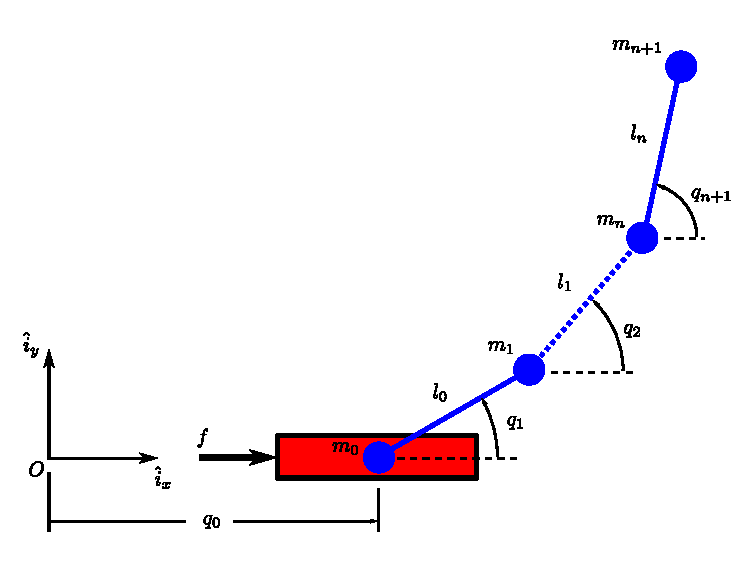
\includegraphics[width=10cm]{n-pendulum-with-cart}
\end{frame}


\begin{frame}
\frametitle{Benchmarks}
\framesubtitle{PyDy Benchmark}
\begin{table}
\begin{tabular}{l | c | c | c  }
n & SymEngine + SymPy & SymPy only & Speedup\\
\hline \hline
10 & 0.17 s & 5.58 s & 32.8x \\
15 & 0.44 s & 22.07 s & 50.1x \\
20 & 0.95 s & 45.59 s & 47.9x \\
30 & 3.11 s & 162.80 s & 52.3x \\
40 & 7.02 s & 427.16 s & 60.8x \\
50 & 13.95 s & 915.83 s & 65.6x \\
60 & 23.16 s & 1596.37 s & 68.9x
\end{tabular}
\caption{Results}
\end{table}
\end{frame}


\begin{frame}
\frametitle{Benchmarks}
\framesubtitle{PyDy Benchmark}
\includegraphics[width=10cm]{pydy}
\end{frame}


\begin{frame}[fragile]
\frametitle{Examples of Usage}
\framesubtitle{Python}

\begin{verbatim}
$ conda install python-symengine --channel conda-forge
$ python
>>> from symengine import *
\end{verbatim}
% add more example scripts above
\end{frame}


\begin{frame}[fragile]
\frametitle{Examples of Usage}
\framesubtitle{Julia}

\begin{verbatim}
julia> Pkg.clone("https://github.com/symengine/SymEngine.jl")
julia> Pkg.build("SymEngine")
julia> using SymEngine
\end{verbatim}
% add more example scripts above
\end{frame}

\end{document}
